%%==================================================
%% chapter02.tex for SJTU Course Design Thesis
%% based on CASthesis, SJTU master thesis
%% modified by icetiny@gmail.com
%% version: 0.3a
%% Encoding: UTF-8
%% last update: Dec 5th, 2010
%%==================================================

% \bibliographystyle{sjtu2} %[此处用于每章都生产参考文献]

\chapter{硬件设计}
\label{chap:hardware}
	本文将主要介绍软件部分的设计,通过对软件设计方案的描述,实现对整个系统功能的介绍。但是硬件部分仍是整个系统的基础,与软件设计也有着密切的关系。本章将对基本的硬件设计做一个浏览。并重点介绍与软件相关最为密切的部分。
\section{硬件设计总体概况}
	本系统采用AT89S52单片机为控制核心,晶振电路产生11.0592 MHz的晶振频率,具有复位电路。输入部分有四个地感线圈信号(接P1口低四位),五个键盘按键输入信号(接P2口高五位)。输出部分驱动六个数码管,六个信号灯,四个拍照驱动信号。图\ref{fig:circuitsmall}是控制部分电路图,附录\ref{app:circuit}图\ref{fig:circuitall}为其放大版。
	
\begin{figure}[!tbh]
  \centering
  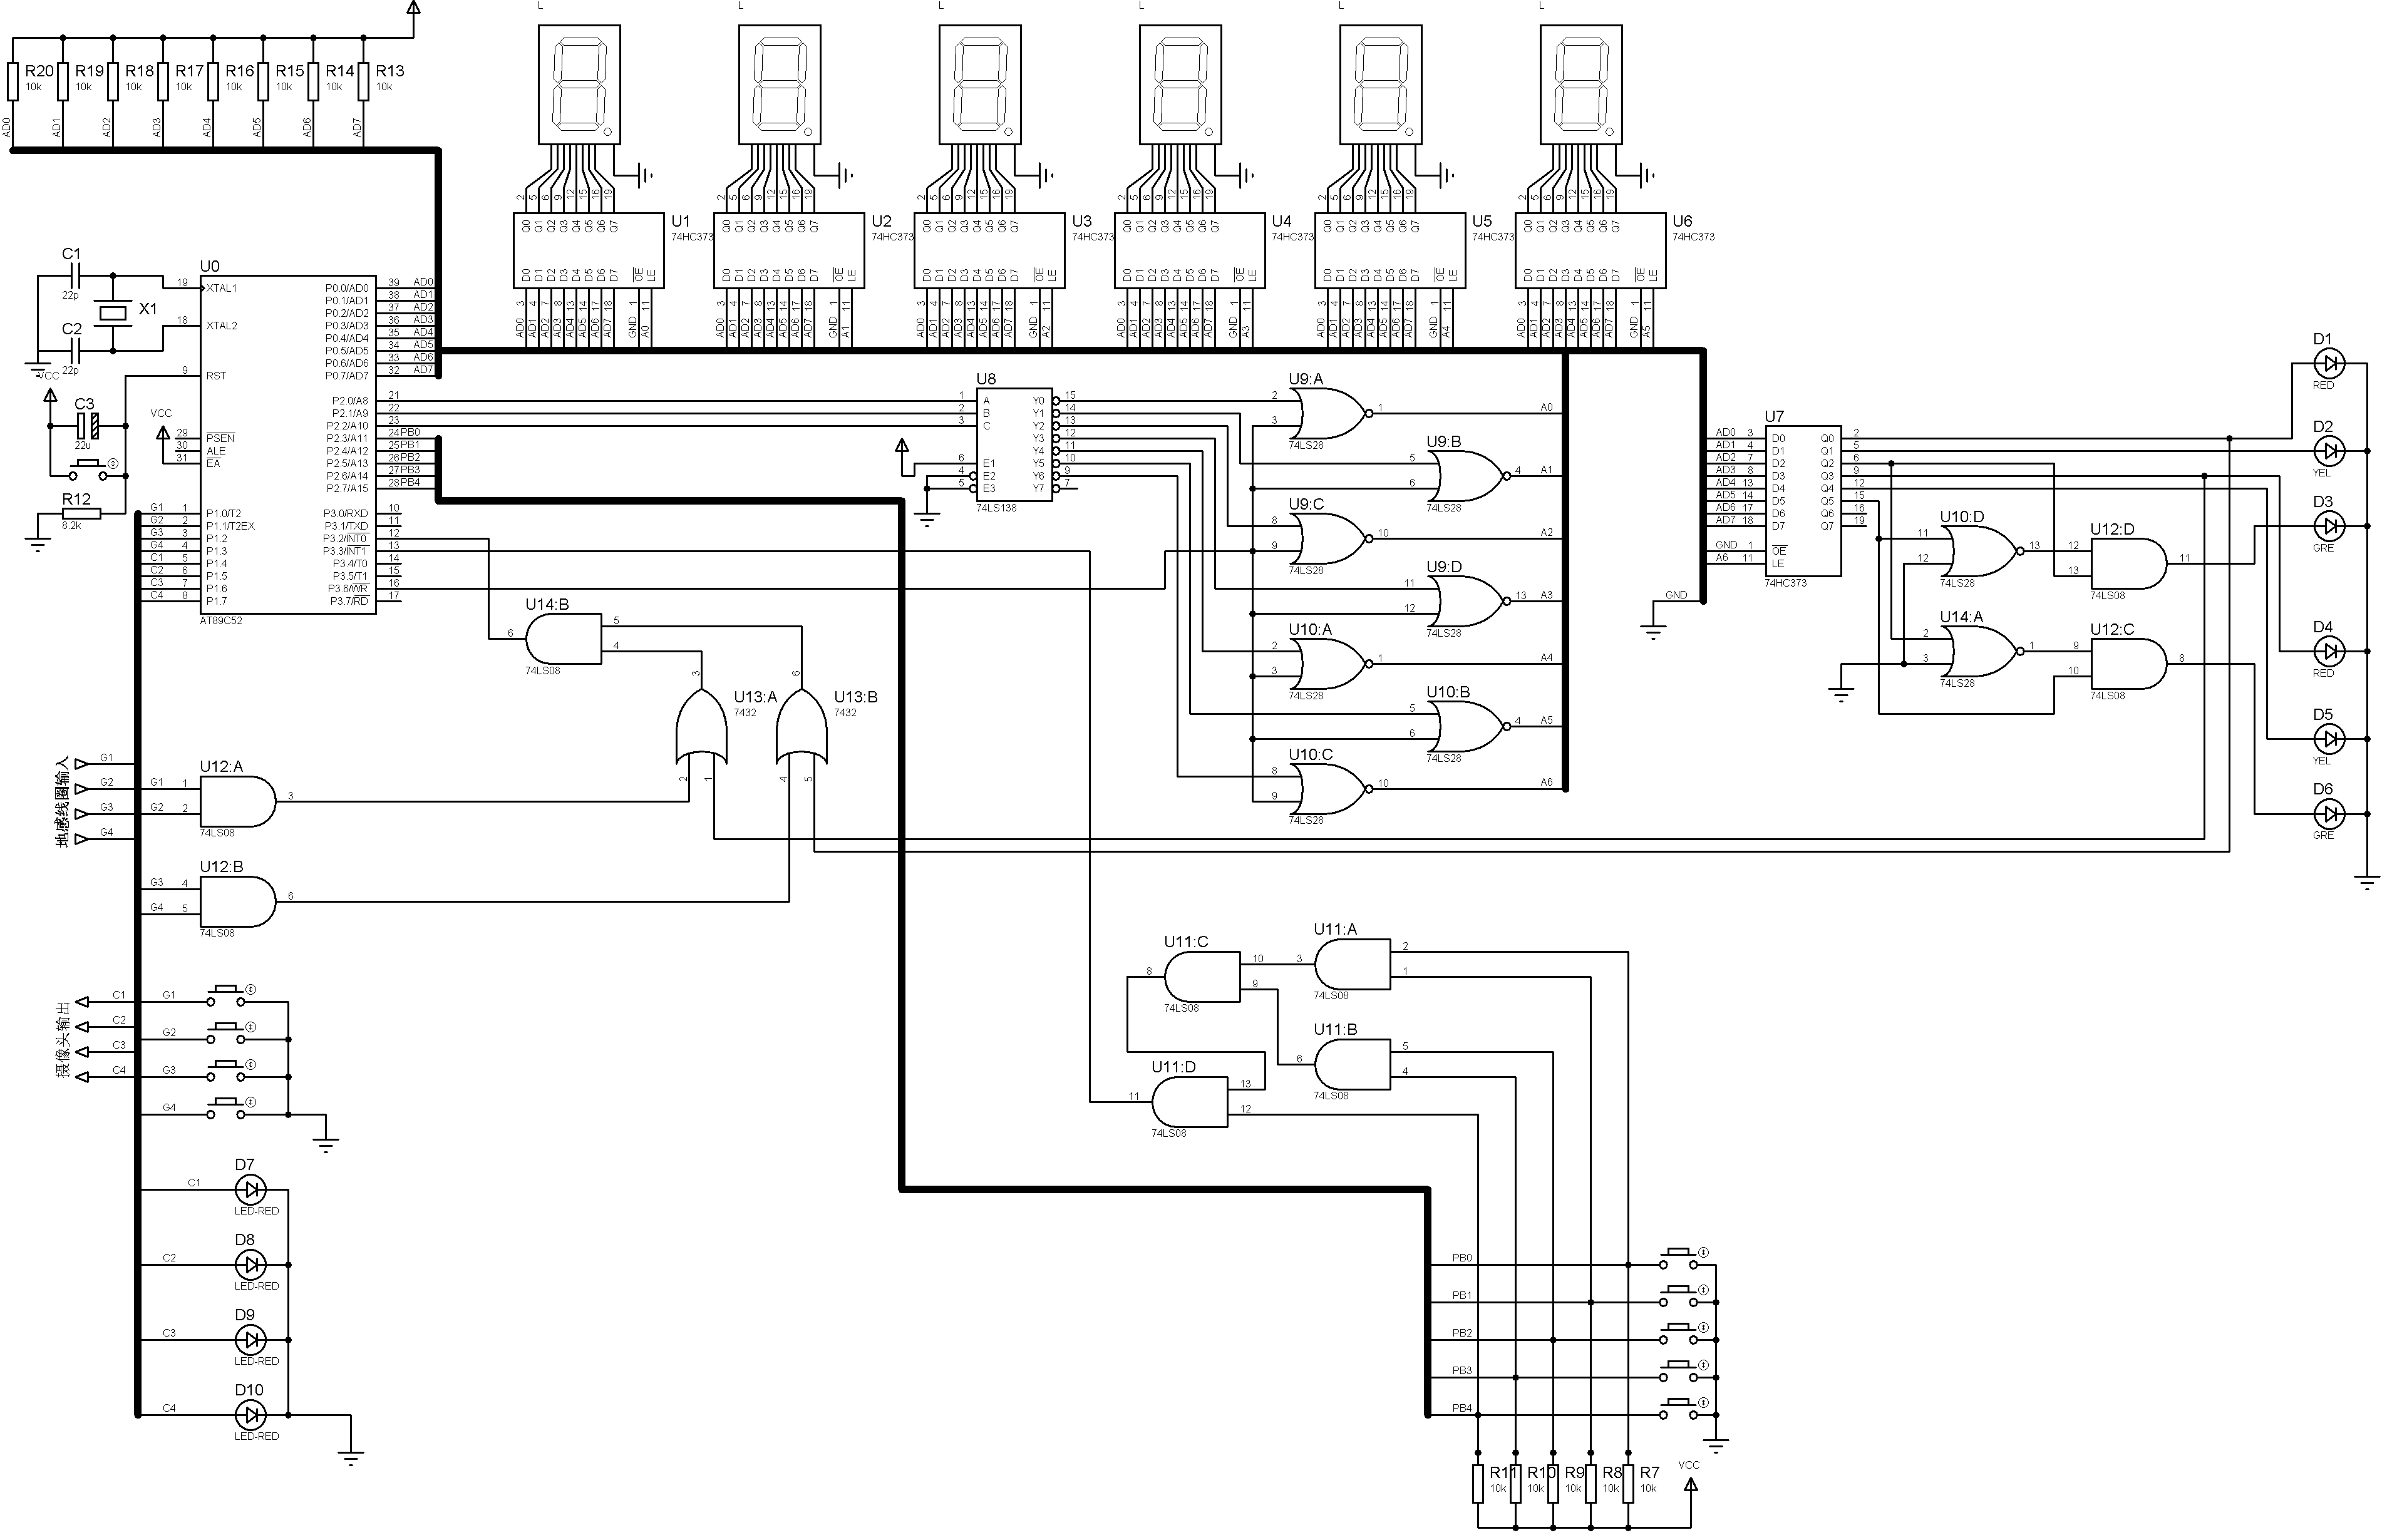
\includegraphics[width=0.85\textwidth]{chap2/circuitsmall.png}
  \bicaption[fig:circuitsmall]{电路图(小)}{控制电路图}{Fig}{Control Circuit Figure}
\end{figure}
	要实现规定的功能目标,通过估算,另外也考虑到S52单片机内部存储器足够大(8K),而最终生成的程序为1.32Kb,RAM空间也有剩余,故不需要进行存储器的扩展。
	
	地感线圈处的输入信号需通过继电器与控制电路连接,具体的连接参数视地感线圈而定。信号灯与数码管的控制信号需要通过光电耦合器后放大再驱动相应器件。这些电路,在以上的控制电路图中并没有体现,但在完整的系统中,它们是同样重要的。
	
\section{数码管及信号灯驱动电路}
	
	\subsection{数码管}
	数码管采用共阴数码管。为了提高显示质量,每一个数码管均通过一个373锁存器驱动,共六个。这样做可以实现静态显示,数码不会闪烁。软件实现也大为便捷,CPU占用率也降低许多。图\ref{fig:hard:digitled}是数码管部分的电路图。
	\begin{figure}[!tbh]
	\centering
	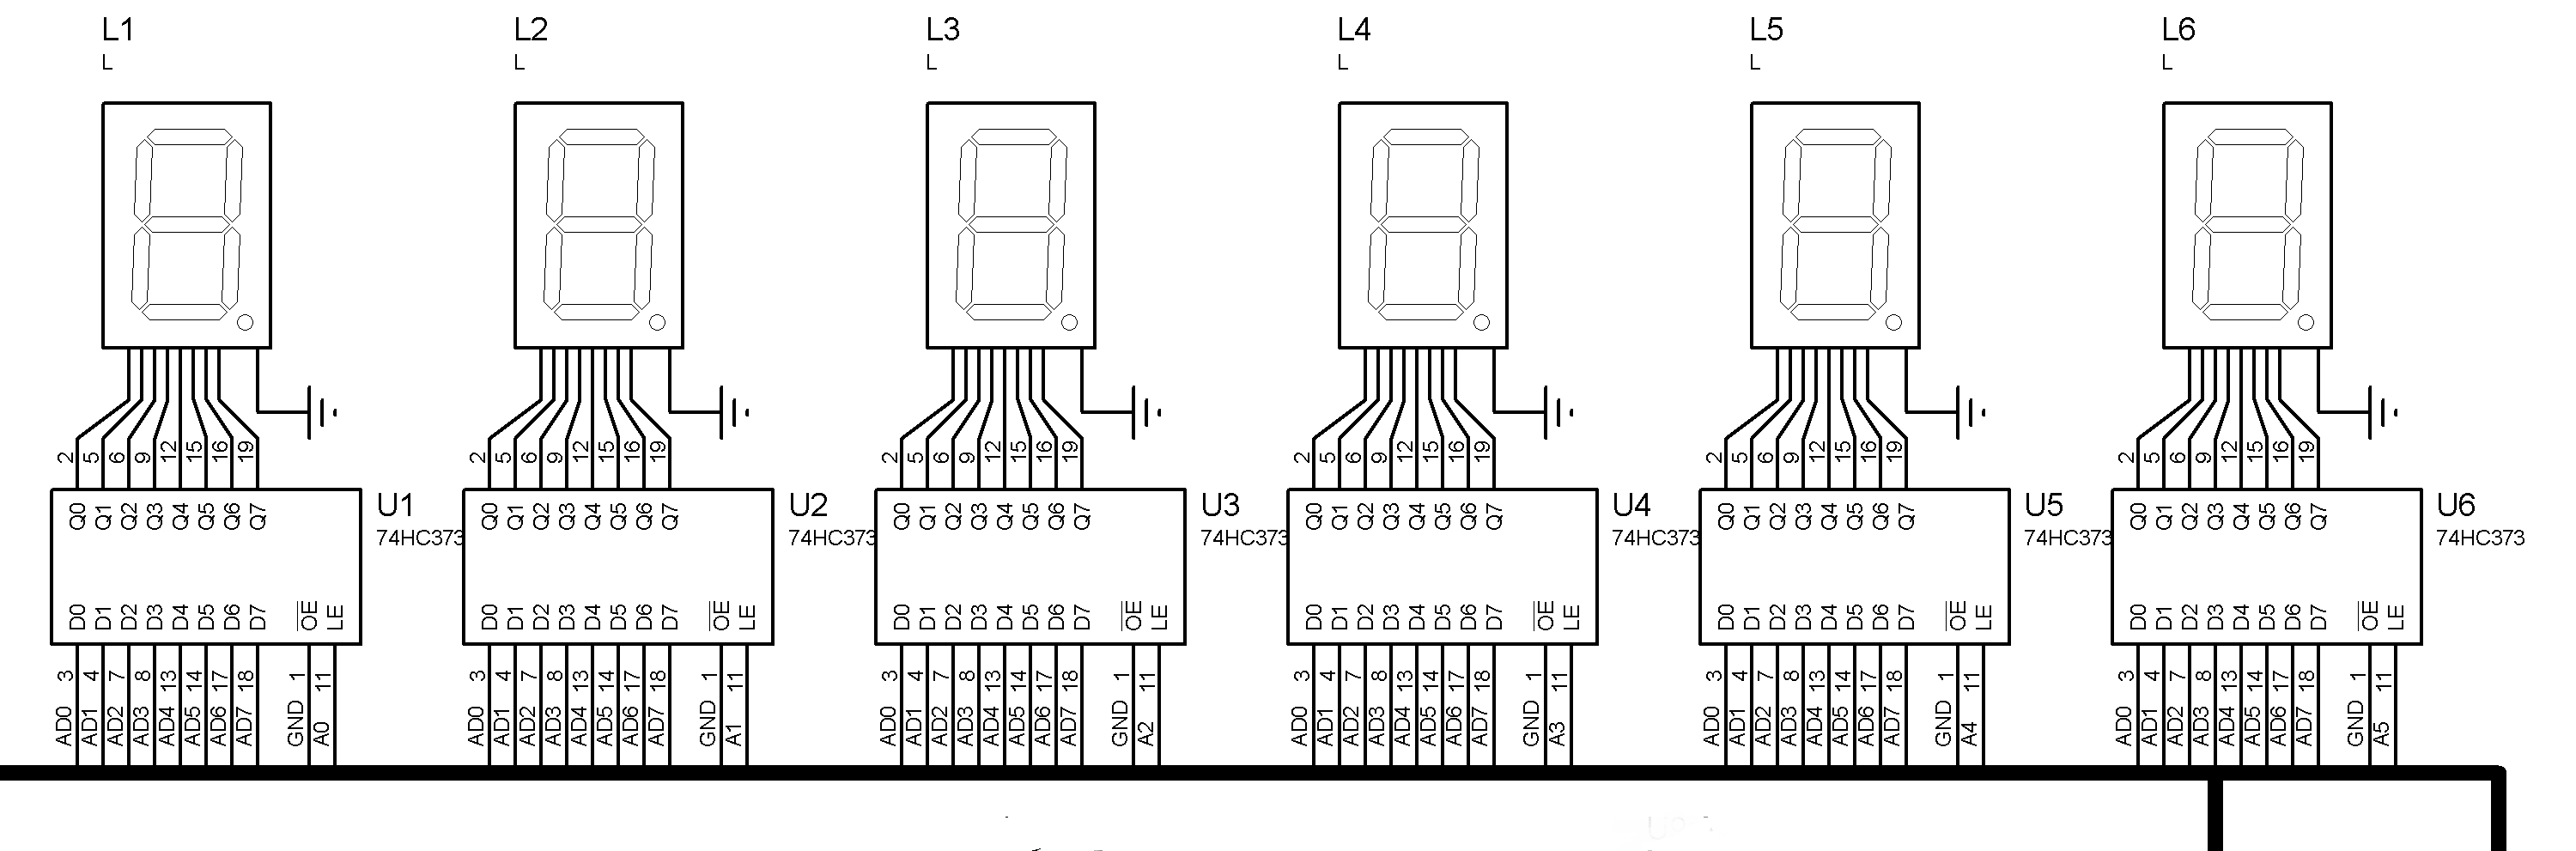
\includegraphics[width=0.7\textwidth]{chap2/digitled.png}
	\bicaption[fig:hard:digitled]{数码管驱动电路}{数码管驱动电路}{Fig}{Digital Led drive circuit}
	\end{figure}
	
	\subsection{信号灯驱动电路} \label{sec:hard:lightbull}
	信号灯驱动电路如图\ref{fig:hard:lightbull}所示。因为相对的路的信号灯内容相同,所以两条路且每条路三盏灯,共六盏灯,通过一个373锁存器驱动。图中可见互锁电路由两个或非门(非门)和两个与门组成,则两个绿灯不能同时点亮。尽管软件中避免了两盏绿灯同时点亮的情况的出现,但硬件互锁还是必不可少的,毕竟软件在运行过程中可能会受到干扰而混乱,可能出现不可预料的情况。
	
	图中所绘的小灯为演示所用,实际应将输出信号放大后,再驱动高电压的信号灯。
	\begin{figure}[!tbh]
	\centering
	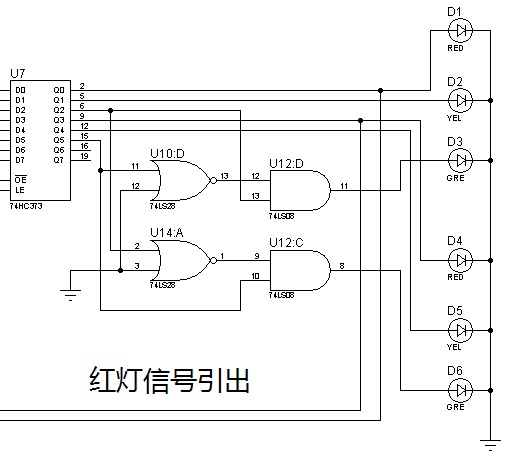
\includegraphics[width=0.6\textwidth]{chap2/lightbull.png}
	\bicaption[fig:hard:lightbull]{信号灯驱动电路}{信号灯驱动电路}{Fig}{Signal light drive circuit}
	\end{figure}
	
	图中还可以看到两个红灯处引出了两路信号,这样做的目的将在\ref{sec:hard:int0}节详细阐述。
	
	\subsection{数码管及信号灯的选通}
	P0口作为数据总线和七个373锁存器相连,P1口的低三位作为地址线,再经过一个38译码器选通各锁存器。单片机的WR信号与38译码器的七个输出端分别或非之后再选通锁存器。在对方案的重新评估中,我们发现也可以令WR信号直接选通138译码器,但考虑到译码器的输出端仍需通过非门,器件数量并未减少太多,故仍保留最初的设计。

\section{键盘}
	图\ref{fig:hard:keyboard}是键盘的电路图。因为P2口正好还有五个IO口可用,五个键也正好可以实现设置的要求,所以采用的独立键盘。这样对于编程工作也是很大的便利。各键的定义在\ref{sec:keydefination}节介绍。
	\begin{figure}[!tbh]
	\centering
	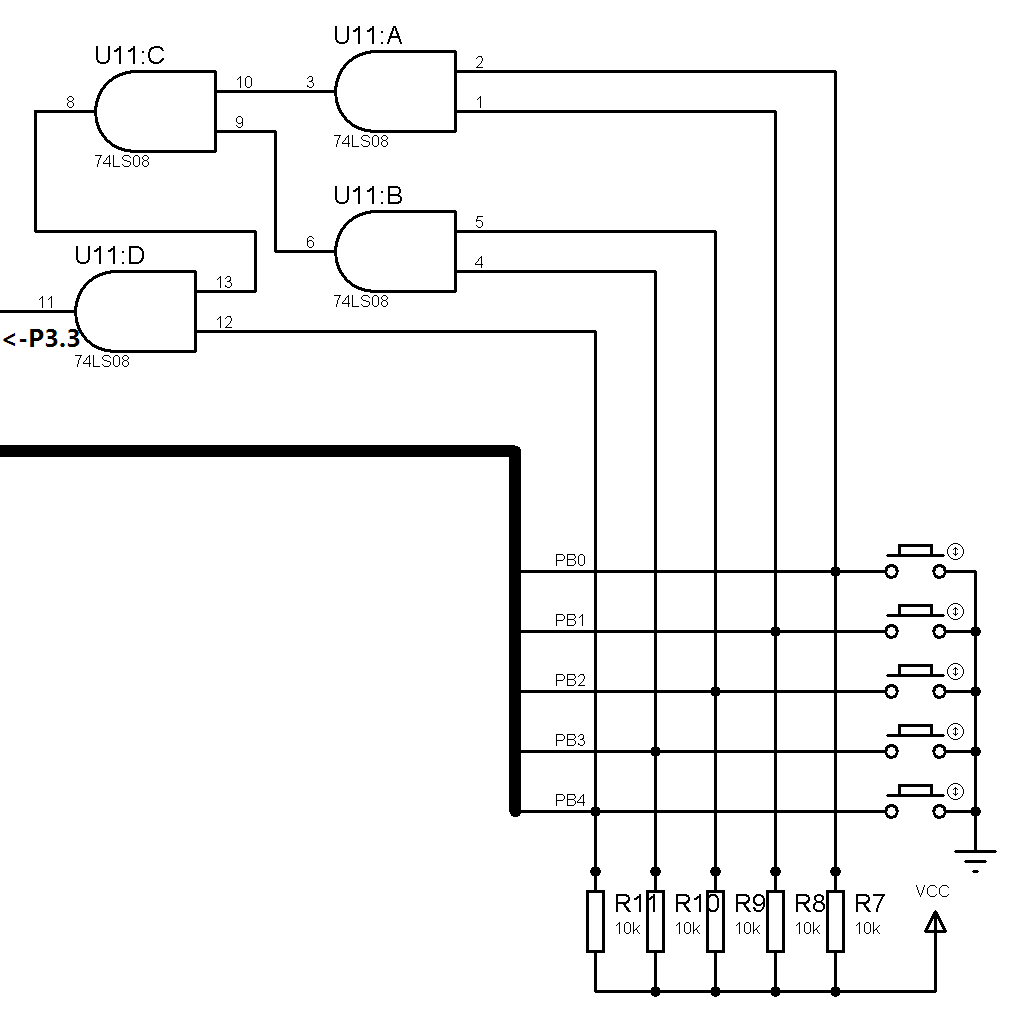
\includegraphics[width=0.5\textwidth]{chap2/keyboard.png}
	\bicaption[fig:hard:keyboard]{键盘电路}{键盘电路}{Fig}{Keyboard circuit}
	\end{figure}
	
	按键触发后P2口有下降沿信号,这个信号全部相与后接P3.3($\bf \overline{INT1}$),可产生中断信号,在软件中再通过轮询确定具体按下的键位。
	
\section{地感线圈输入与中断触发} \label{sec:hard:int0}
	地感线圈输入信号送入P1口低三位,并触发$\bf \overline{INT0}$中断。在电路图中地感线圈的输入以开关代替,实际信号也是一开关量,但由地感线圈转换至单片机控制电路输入信号还需要一些处理。
	
	\begin{figure}[!tbh]
	\centering
	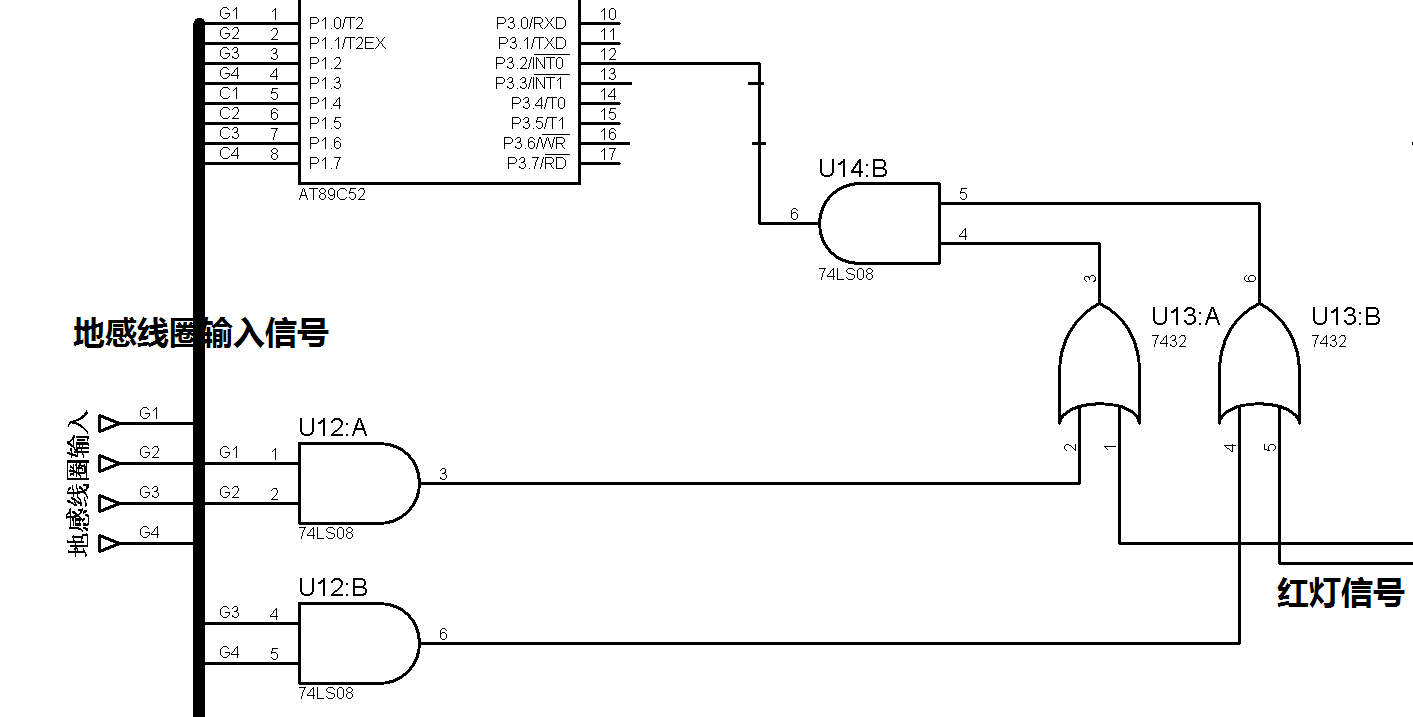
\includegraphics[width=0.7\textwidth]{chap2/redint0.png}
	\bicaption[fig:hard:redint0]{地感线圈输入电路}{地感线圈输入电路}{Fig}{Ground wire input}
	\end{figure}
	
	由图\ref{fig:hard:redint0}可见,此电路与普通的外部中断扩展电路稍有不同,在\ref{sec:hard:lightbull}节已提到,两路红灯信号由右侧引入,分别与另一条路的地感线圈输入信号取或运算,然后在送入$\bf \overline{INT0}$口。这是为了在某一路为绿灯时,屏蔽其地感线圈的信号,使之不能产生中断。只有在某一路为红灯时,闯红灯的车辆才能触发地感线圈,继而触发单片机中断。这样大大减少了中断的产生大大降低了CPU的工作量,提高了反映速度。编程难度也有所减轻。

\section{小结}
除了以上介绍的主要输入输出电路外,我们还设计了上电复位电路,晶振频率为11.0952MHz的时钟电路,P0口加入了上拉电阻。由于这些电路都较为常规,在此不再详述。

通过以上的分析可见,我们的设计对单片机IO口的利用非常充分P0,P1,P2口均已占满。通过充分利用IO口实现了数码管和信号灯的静态显示、独立键盘、独立的地感线圈输入,减少了元器件的使用,减小了编程难度。

硬件电路设计中也通过一些逻辑电路的组合,实现了互锁、条件屏蔽等功能。